\chapter{Konzept}
\label{chap:konzept}

Dieses Kapitel beschreibt die konzeptionellen Überlegungen der Lösung. Als erstes werden die grundlegenden Begriffe erklärt, welche in den darauf folgenden Kapiteln verwendet werden. Das Zusammenspiel der einzenen Komponeten und der Aufbau der MQTT Topic Hierarchie werden erläutert. 

\section{Allgemein}

Um ein \gls{iot} Systeme zu realisieren, sind viele Komponenten nötig, welche miteinander interagieren müssen. In diesem wird Abschnitt beschrieben, aus welchen Teilen ein solches System besteht und welche Teile die Beschreibung eines Devices enthalten soll.

\textbf{Device} \\
Sensoren und Aktoren werden unter dem Begriff Device zusammengefasst.


\textbf{IoT Gateway} \\
Die einzelnen Devices eines \gls{iot} Systems sind an einen Gateway angeschlossen. Dies kann fix per Kabel oder über eine Drahtlosschnittstelle wie z. Bsp. Bluetooh umgesetzt sein. Typsicherweise werden Kleincomputer (Single Board Computer) wie ein Raspberry Pi oder Intel Galileo eingesetzt. Diese Geräte zeichnen sich aus durch sehr kompakte Bauform (Kreditkatenformat) und bieten trotzdem genügend Ressourcen um darauf hardwareunabhängige Anwendungen (z. Bsp. Java, Python, Javascript) laufen zu lassen. 
Ein Gateway führt die Daten der einzelnen Devices zusammen und vereinheitlicht die Formate der Daten. Ausserdem übernimmt er die Kommunikation mit der Aussenwelt, indem er eine Verbindung zum MQTT Broker herstellt.

\begin{figure}[H]
	\centering
		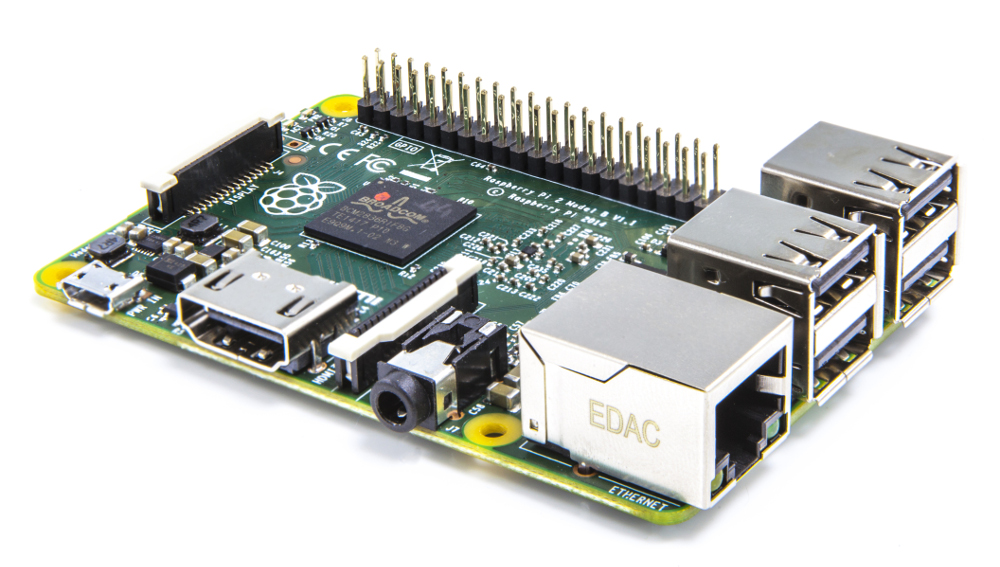
\includegraphics[width=0.6\textwidth]{bilder/raspi_2.jpg}
	\caption{Beispiel eines Gateways: Raspberry Pi 2}
\end{figure}

\textbf{MQTT-Broker} \\
Der Broker ist bei \acrshort{a_mqtt} Anwendungen von zentraler Bedeutung, da alle Daten via Broker zwischen den Teilnehmern ausgetauscht werden. Pro System gibt es typischerweise einen Broker. Dieser muss für alle Teilnehmener (Gateways und Applikationen) einfach zu erreichen sein und eine hohe Verfügbarkeit aufweisen.

\textbf{Applikation} \\
Es können grundsätzlich beliebige Applikationen auf allen gängigen Platformen und Technologien mit den System kommunizieren. Die einzige Grundbedingung ist, dass die Applikation \acrshort{a_mqtt} fähig ist, was sich durch das Einbinden der entsprechenden Libraries einfach realisieren lässt.
\\


\textbf{Device Description} \\
Ein Device wird als ganzes mit einen Schema beschrieben. Die Device Description wird als retained MQTT Message beim Start des Devices resp. Gateways an den Broker geschickt.

Eine Device Description enthält folgende Hauptbereiche:

\textbf{State} \\
Die Menge aller Eigenschaften des Devices und deren Werte werden als State bezeichnet. Beispielsweise Name, Firmwareversion, etc. Der State eines Devices ist beständig, d.h. solange keine Interaktion statfindet , verändert sich der State nicht.


\textbf{Events} \\
Tritt auf dem Device ein Ereignis ein, wird dadurch ein Event erzeugt. Ein Event wird grundsätzlich vom Device selbst ausgelöst. Beispielsweise erzeugt ein Temperatursensor alle 5 Sekunden ein Event welches den Messwert enthält. Applikationen registrieren sich, um bestimmte Events von den Devices zu erhalten.


\textbf{Commands} \\
Eine Applikation interagiert mit einem Device, indem Commands an eines oder mehrere Devices gesendet werden. Die Devices empfangen die Commands und reagieren entsprechend. Ein Command ist bestimmt durch einen Namen und Parameter mit dazugehörigen Werten. 
Beispielsweise kann bei einem Temperatursensor über einen Command \code{SetInterval: 10s} der Abstand der Messungen eingestellt werden.
Ein Device muss bekanntgeben, auf welche Commands mit welchen Paramtern es reagiert.


\begin{figure}[H]
	\centering
		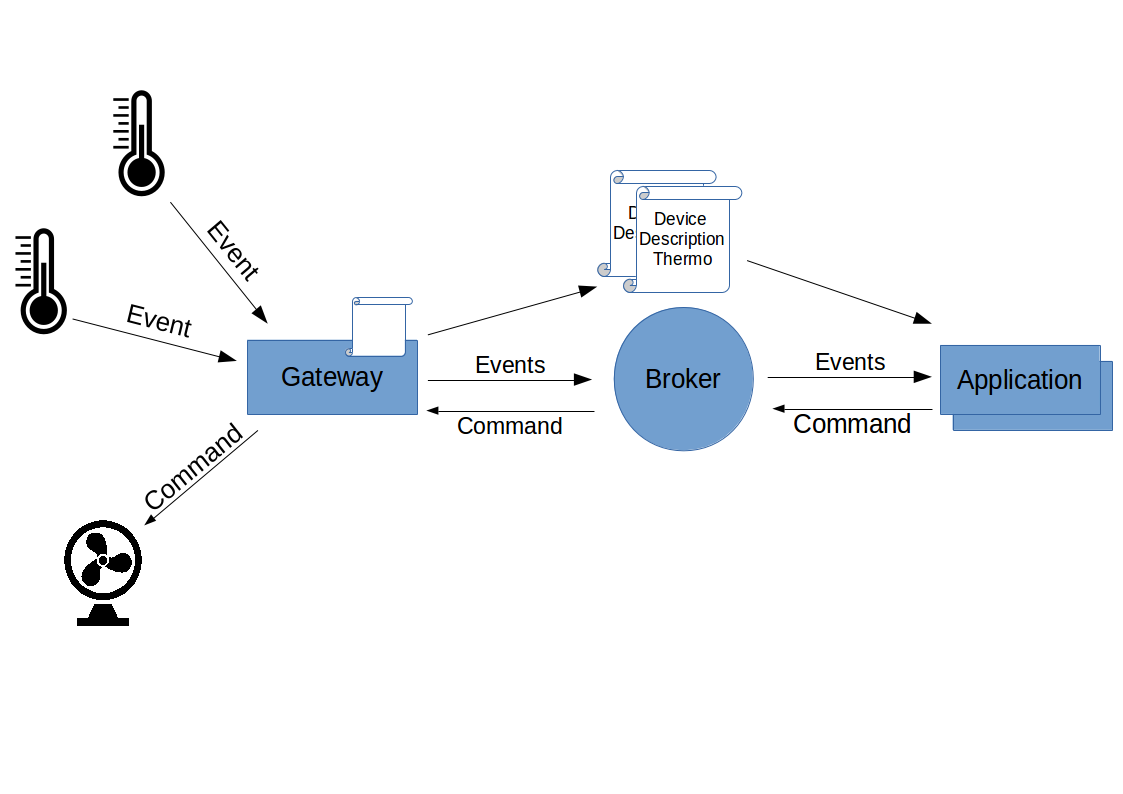
\includegraphics[width=0.8\textwidth]{diag/Overview.png}
	\caption{\label{fig:overview}Systemübersicht}
\end{figure}


\section{Datenformate}
Das System wird so konzipiert, dass es möglich ist, die Daten in verschiedenen Formaten zu codieren für das Versenden der Messages. Für die Umsetzung wird das Format YAML eingesetzt. Die einfache Lesbarkeit des Formats ist während der Entwicklung bei häufigen Änderungen von grossem Vorteil.

\newpage

\section{Hierarchie Topics}

Die Topic Hierarchie wird nach folgenden Muster aufgebaut:

\begin{figure}[H]
	\centering
		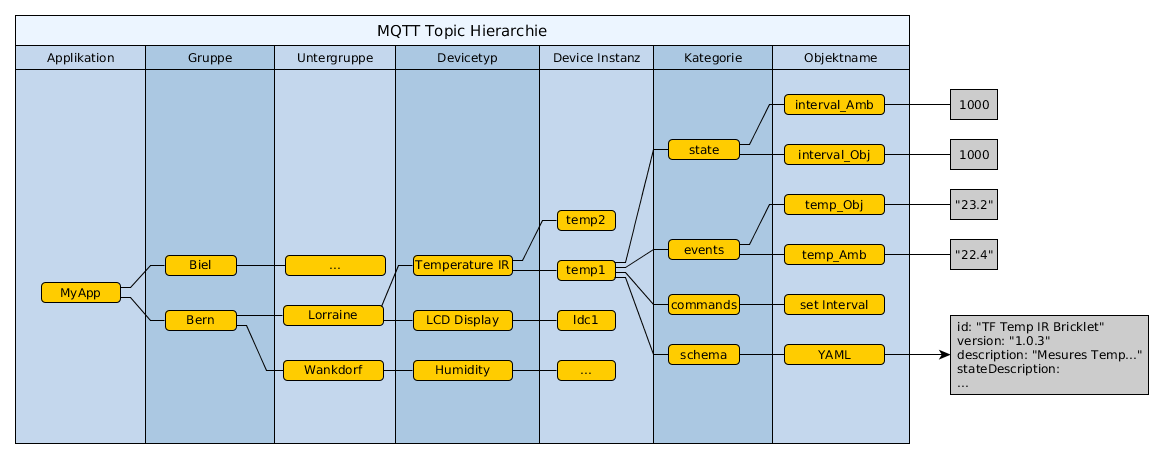
\includegraphics[width=1.0\textwidth]{diag/topic_hierarchy.png}
	\caption{\label{fig:tempitTopics}Aufbau MQTT Topics mit Beispieldaten}
\end{figure}


\begin{table}[H]
\begin{tabularx}{\textwidth}{|l|X|l|}

 \hline \rowcolor{lightgray}
 {\bf Level } & {\bf Beschreibung } & {\bf Beispiel } \\ 
 \hline
 0  &   \textbf{Applikation} \newline Identifikation der Anwendung.  &    
  thesisDemo   \\ \hline
 
 1  &   \textbf{Gruppe}  \newline Gruppierung der Devices auf Stufe 1 &   Bern  \\ \hline

 2  &   \textbf{Untergruppe} \newline Gruppierung der Devices auf Stufe 2   &   Lorraine  \\ \hline

 3  &   \textbf{Devicetyp} \newline Bezeichnung, um was für einen Typ von Sensor oder Aktor es sich handelt.  &   Temperatursensor   \\ \hline

 4  &   \textbf{Device Instanz} \newline Da mehrere Devices vom selben Typ im Einsatz sein können, wird auf dieser Stufe mit einer eindeutigen ID der konkrete Sensor resp. Aktor angegeben.   &    temp1   \\ \hline
 
 5  &   \textbf{Kategorisierung Devicedaten} \newline  Die Eigenschaften und Daten werden in die nachfolgenden Teile aufgegliedert.  &     state, events, commands, schema   \\ \hline
 
 6  &   \textbf{Objektname} \newline Name es State, Events oder Commands    &     temp\_Obj   \\ \hline

 6  &   \textbf{Schema Format} \newline Als Unterobjekt von 'schema', wird hier das Format des Schemas angegeben   &     YAML, JSON   \\ \hline
 

\end{tabularx}
\caption{Topic Hierarchie}
\end{table}


\section{Abgrenzung}

\subsection{Security}
Betrachtungen zum Thema Security werden in dieser Arbeit nicht behandelt. Es wird davon ausgegangen, dass alle Teilnehmer des Systems dazu berechtigt sind und innerhalb des Systems nur Nachrichtenaustausch nach dem beschriebenen Konzept stattfindet.

\subsection{Optimierungen Datenmenge}
Bei der Strukturierung der Device Topic Hierarchie und dem Format der Payload Daten (Schema, State, etc.) ist im Rahmen dieser Arbeit Verständlichkeit und Übersichtlichkeit höher priorisiert als die Optimierung auf möglichst geringe Datenmengen.